\chapter{Destructive 3D phenotyping pipeline}

\section{Introduction}

Estimating the plant phenotypes accurately and efficiently can help to bridge the gap between genotype and phenotype. The traditional phenotyping measurement is time-consuming, laborious, and often not accurate. Although several authors have developed 2D image-based phenotyping methods which are more efficient, non-destructive, and have higher throughput \citep{yang_greenness_2015,guo_easypcc_2017,zou_broccoli_2019}, these approaches are unable to describe the plant 3D structure due to the occlusion and dimension loss when projecting onto the 2D plane. As a result, it produces inaccuracies and uncertainties for advanced phenotyping applications.

To overcome the drawbacks of 2D image-based phenotyping, several studies have paid attention to 3D approaches. \citet{paulus_measuring_2019} and \citet{kochi_introduction_2021} have summarized the current approaches to obtain 3D plant models, and a large number of studies have chosen the 3D reconstruction by photogrammetry using common RGB cameras due to the low device cost \citep{xiao_estimating_2021,zermas_3d_2020,zhang_estimating_2016}. The key idea of sfm, was taking images from different angle views and calcualting their relative positions to object.

% the key idea of sfm, and the classes of sfm


\begin{figure}[htb]
  \begin{center}
    \resizebox{\textwidth}{!}{
      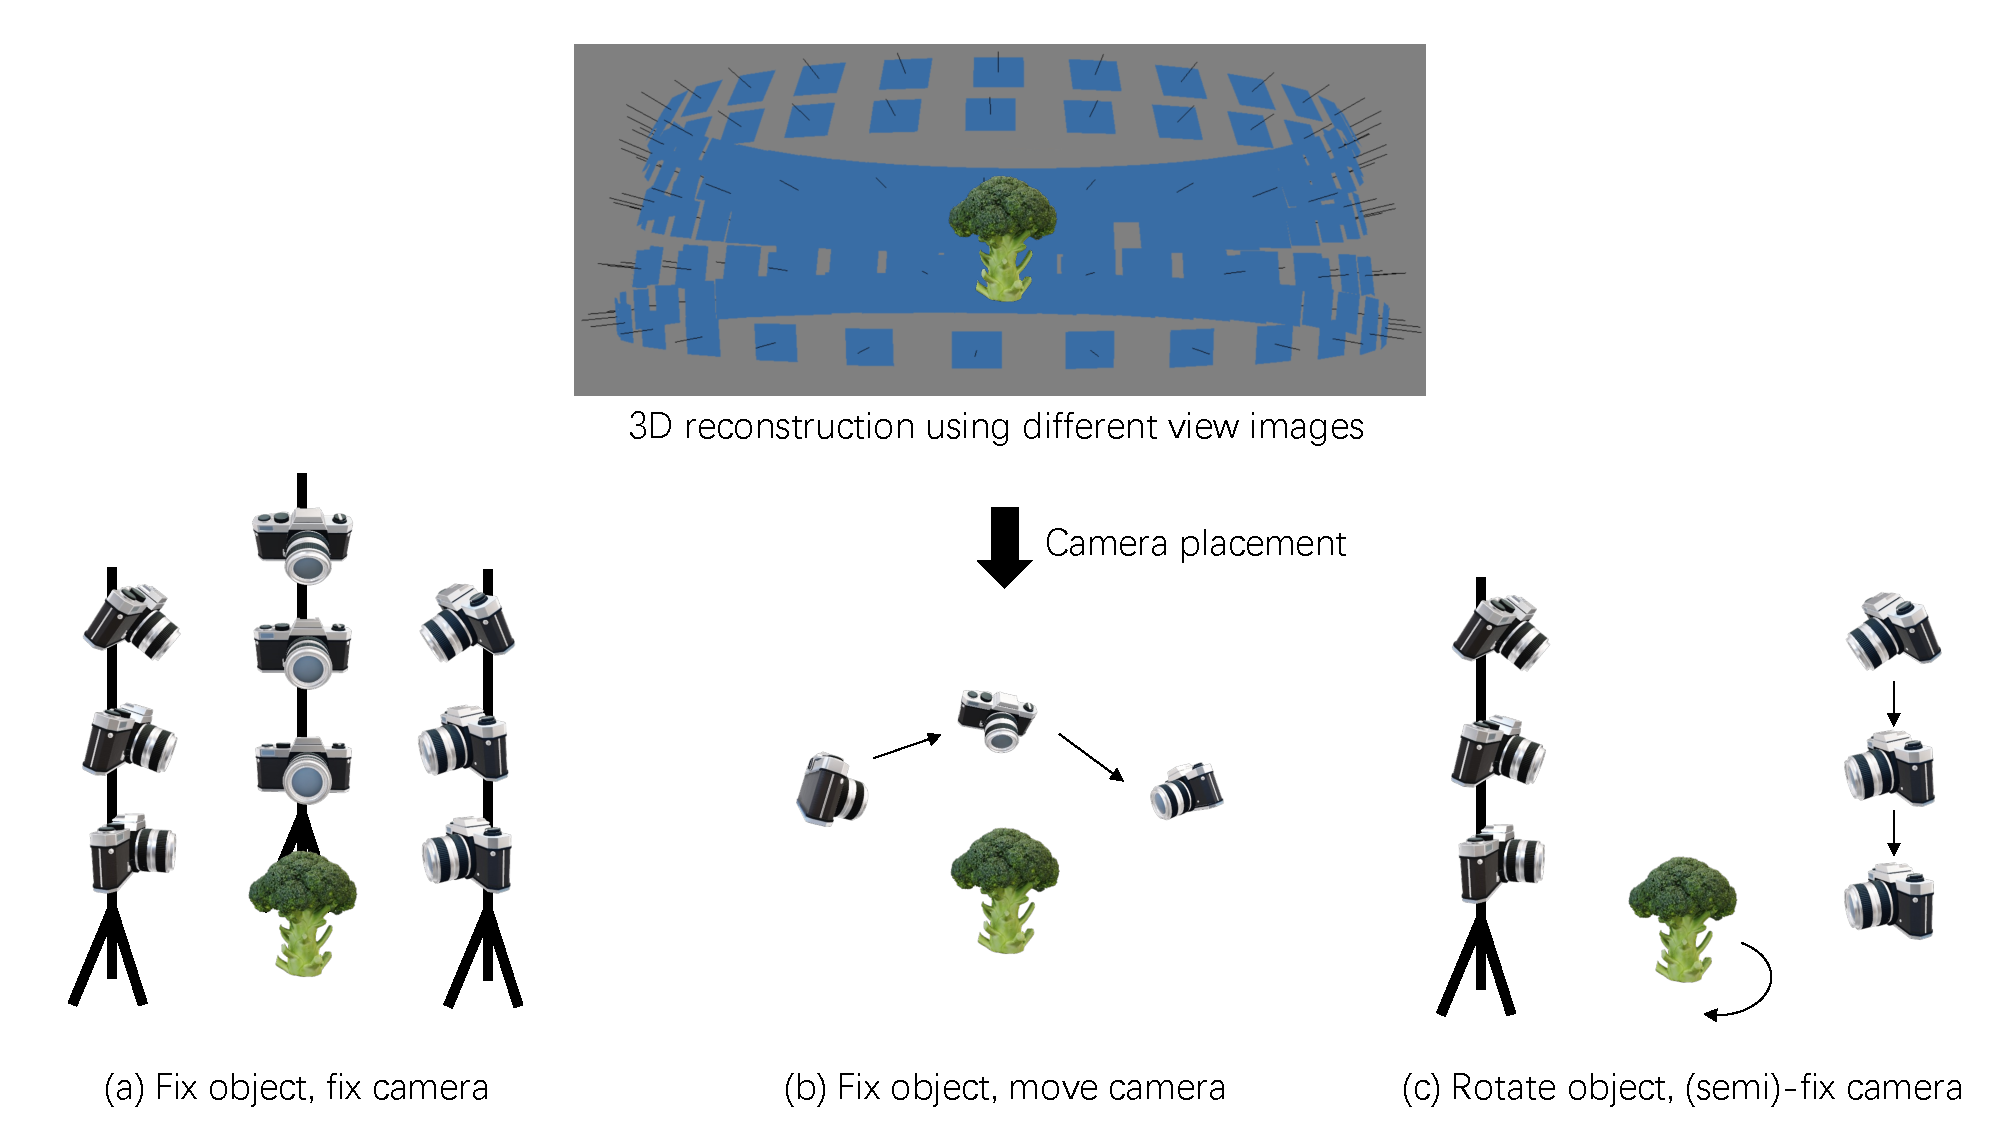
\includegraphics{figures/des/sfm_types.pdf}
    }
  \end{center}
  \caption[Current photogrammetry (3D reconstruction) methods and challenges]{
    The current photogrammetry (3D reconstruction) methods and challenges; (a-c) the current image acquisition approaches (a) fixing the object and taking images using multiple fixed cameras at the same time, also called forward intersection; (b) fixing the object but taking images by using a moved camera, also called backward resection; and (c) rotating the object and taking images using fewer multiple fixed cameras, or a camera fixed at different locations for each rotation. The challenges of current approaches: (d) the limited view angles of current image occlusion approaches has visual dead area, which will cause incomplete plant 3D models; and (e) the difficulties to segment foreground (plant) area in the image preprocessing.
  }
  \label{fig:des1}
\end{figure}


\section{Methods and Materials}




\section{Results}



\section{Discussion}



\section{Conclusion}